\documentclass[11pt]{article}
\usepackage[margin=0.7in]{geometry}
\usepackage{graphicx} %figures
\usepackage{titling}
\usepackage{color}
\usepackage{comment}
\usepackage[none]{hyphenat} %surround text in {} to prevent hyphenation
\usepackage{multirow} %helps tables
\usepackage{array} %helps tables
\usepackage{url}
\usepackage{enumitem}
\usepackage{bold-extra} %allows using small caps and bold series in the same time (use case)

%squeezed itemize for table.
\newenvironment{packed_itemize}{
\begin{itemize}
 % \setlength{}{0pt}
  \setlength{\itemsep}{1pt}
  \setlength{\parskip}{0pt}
  \setlength{\parsep}{0pt}
}{\end{itemize}}



\newenvironment{usecase}{%
	%\def\title$$1{  {\Large\bf{Use Case} ##1} \\}
	\def\title##1{ {\large \bfseries  \scshape {Use Case:} ##1} \\ }
 	\def\id##1{{\bf Indentifier:} ##1\\}
	\def\des##1{ {\bf Description:} ##1\\}
	\def\actors##1{ {\bf Actors:} ##1\\}
    	\def\pre##1{ {\bf Preconditions:} ##1 \\} %
    	\def\flow##1{ {\bf Flow of Events} ##1}%
    	\newenvironment{ucenum}{%
        	\begin{enumerate}[nolistsep]\small}%
        	{\end{enumerate}}
	\def\post##1{ {\bf Postconditions:} ##1 \\}
}{\vspace{.05in}}

\title{YAExs Elaboration}
\author{TimeFinders: Andrew Karnani, Auston Sterling, Jeffrey Rodowicz and Vera Axelrod}
\date{October 11, 2012}

\begin{document}
\maketitle
\tableofcontents
\vspace{0.2in}
\hrule
\vspace{1in}

%%%%%%%%%%%%%%%%%%%%%%%%%%%%%%%%%%%%%%%%%%%
%%%%%%%%%%%%%%%%%%%%%%%%%%%%%%%%%%%%%%%%%%%
\section{Domain Model Diagram} %VERA
Our domain model diagram is shown in Figure \ref{fig:Domain}.  Students take exams in rooms. Exams are scheduled by the Registrar, which takes requests for exams from department schedulers, who in turn collect exam preferences from the instructors who give the exams. At RPI each academic department has an administrator known as a  department scheduler is an administrator who works with the Registrar to coordinate exams.
\begin{figure}
	\centering
		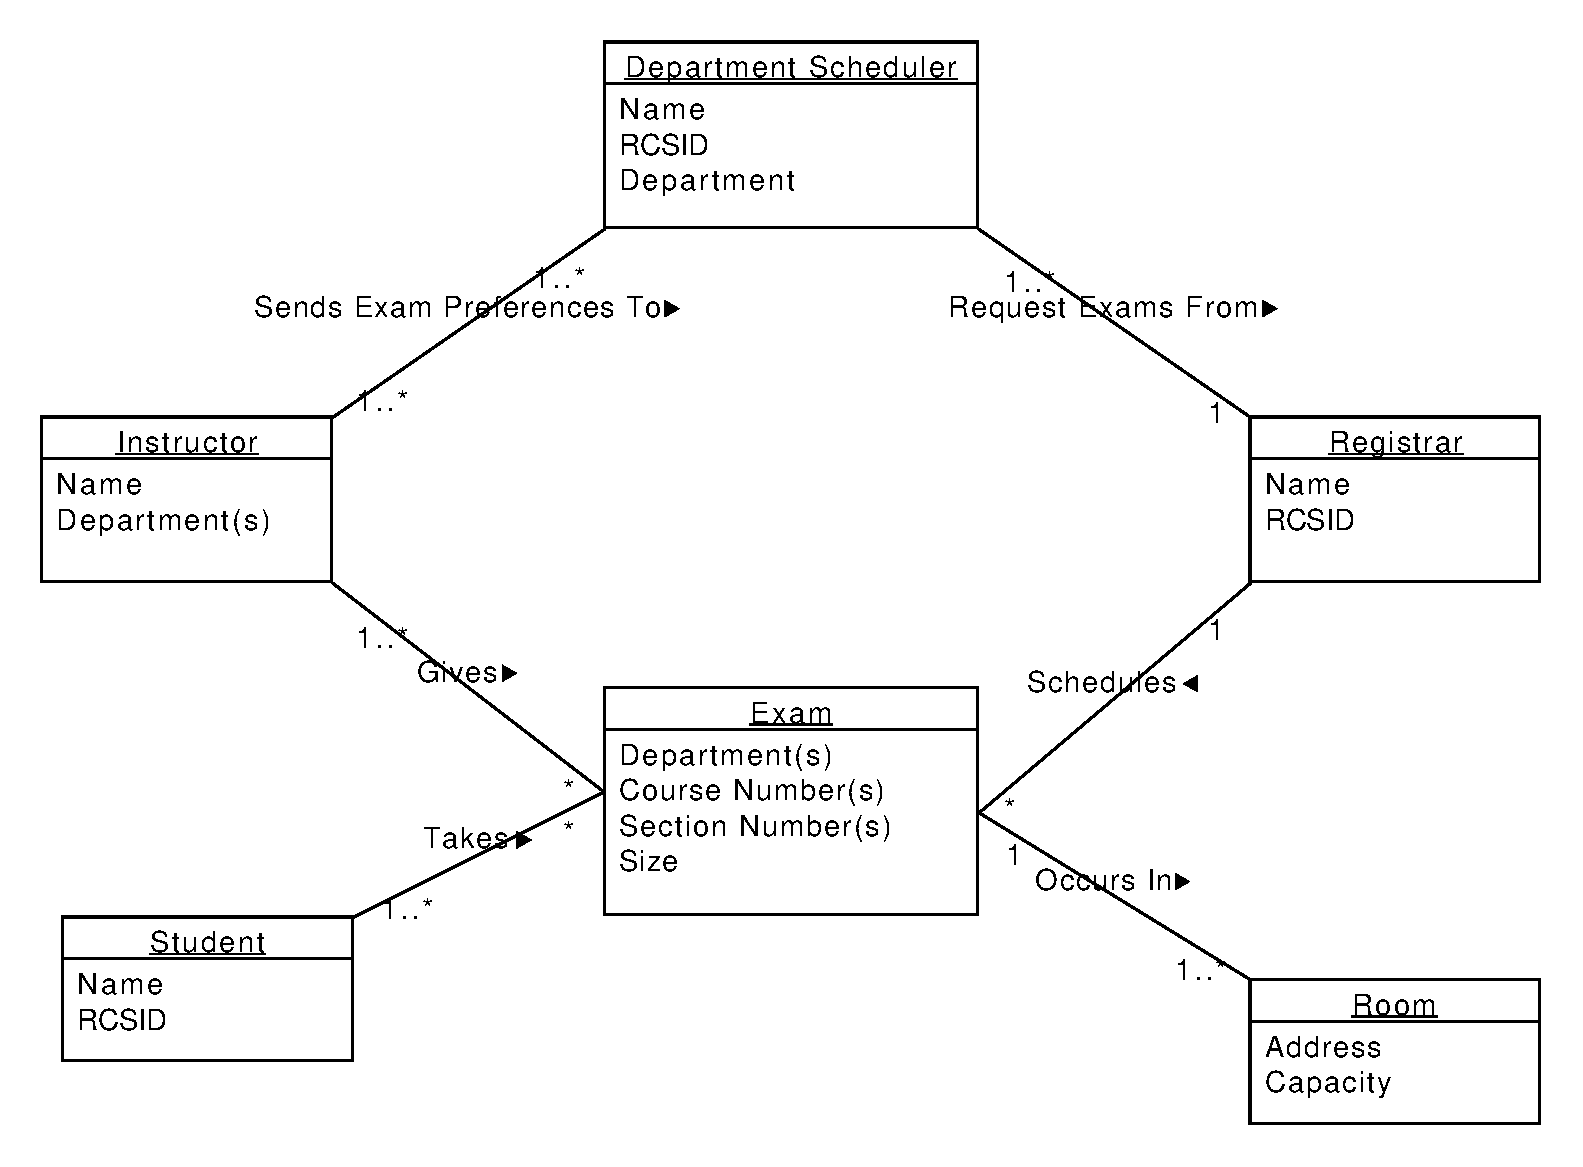
\includegraphics[width = \textwidth]{domainDiagram.pdf}
	\caption{Domain Model}
	\label{fig:Domain}
\end{figure}

%%%%%%%%%%%%%%%%%%%%%%%%%%%%%%%%%%%%%%%%%%%
%%%%%%%%%%%%%%%%%%%%%%%%%%%%%%%%%%%%%%%%%%%
\section{Supplemental Specification} %AUSTON  and ANDREW
%need to make sure everything is connected to a use case


\begin{tabular}{|m{1in}|m{0.3in}|m{0.6in}|m{4.5in}|}
\hline
\textbf{Category}  & \textbf{ID}  & \textbf{Priority}        & \textbf{Description} \\
\hline\hline
%%%%%%%%%%%%%%%%%%%%
\multirow{3}{*}{Functionality }
 & F01 & Must
 & Description \\  \cline{2-4}
%%%%%
 & F02 & Should
 & Description \\  \cline{2-4}
%%%%%
 & F03 & Could
 & Description \\ \hline

%%%%%%%%%%%%%%%%%%%%
\multirow{3}{*}{Usability }
 & F04 & Must
 & Description \\  \cline{2-4}
%%%%%
 & F05 & Should
 & Description \\  \cline{2-4}
%%%%%
 & F06 & Could
 & Description \\ \hline

%%%%%%%%%%%%%%%%%%%%
\multirow{3}{*}{Reliability }
 & F07 & Must
 & Description \\  \cline{2-4}
%%%%%
 & F08 & Should
 & Description \\  \cline{2-4}
%%%%%
 & F09 & Could
 & Description \\ \hline


%%%%%%%%%%%%%%%%%%%%
\multirow{3}{*}{Performance }
 & F07 & Must
 & Description \\  \cline{2-4}
%%%%%
 & F08 & Should
 & Description \\  \cline{2-4}
%%%%%
 & F09 & Could
 & Description \\ \hline

%%%%%%%%%%%%%%%%%%%%
\multirow{3}{*}{Maintainability}
 & F07 & Must
 & Description \\  \cline{2-4}
%%%%%
 & F08 & Should
 & Description \\  \cline{2-4}
%%%%%
 & F09 & Could
 & Description \\ \hline

%%%%%%%%%%%%%%%%%%%%
\multirow{3}{*}{Configurability}
 & F07 & Must
 & Description \\  \cline{2-4}
%%%%%
 & F08 & Should
 & Description \\  \cline{2-4}
%%%%%
 & F09 & Could
 & Description \\ \hline
\end{tabular}

\textcolor{red}{Constraints?}

%%%%%%%%%%%%%%%%%%%%%%%%%%%%%%%%%%%%%%%%%%%
%%%%%%%%%%%%%%%%%%%%%%%%%%%%%%%%%%%%%%%%%%%
\clearpage
\section{Deployment Diagram} %ANDREW

Our deployment diagram is shown in Figure \ref{fig:Deploy}.

\begin{figure}[ht]
	\centering
		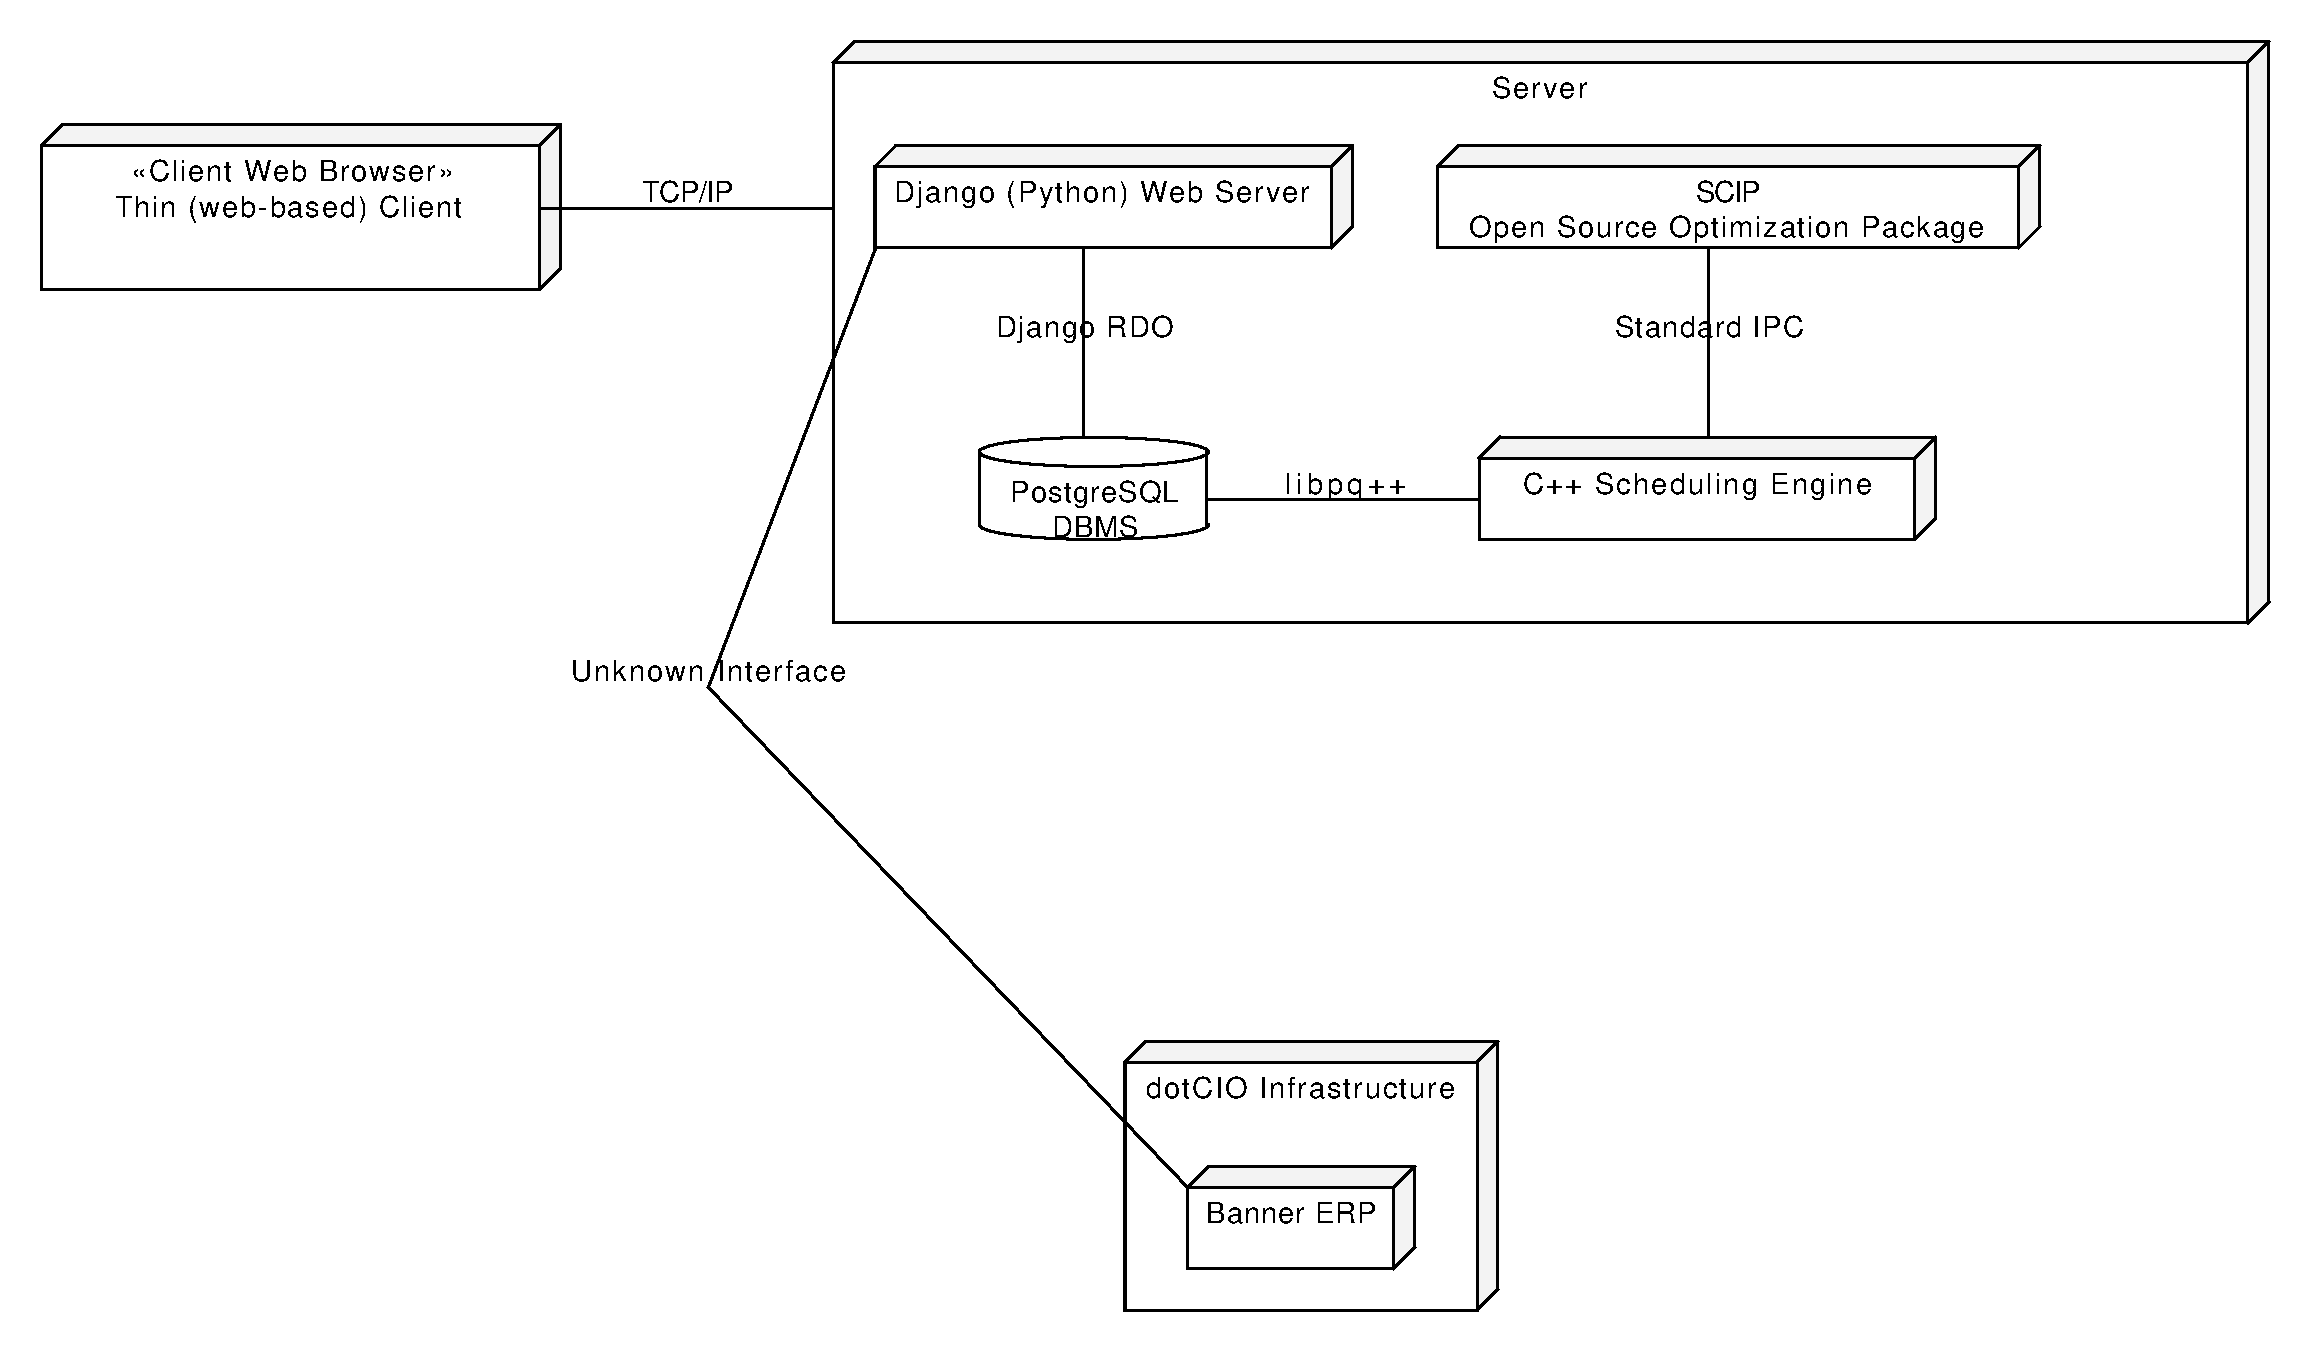
\includegraphics[width = \textwidth]{deploymentdiagram.pdf}
	\caption{Deployment Diagram}
	\label{fig:Deploy}
\end{figure}

YAExS will be a web based application, therefore, the client for the application will be a web browser.  A users's web browser will contact the server via a TCP/IP socket (handled by the browser).  The incoming HTTP request will be handled by Django.  Django will be responsible for gathering information from users and inserting that information into the database.  Django will also interface with Banner (RPI's ERP) to gather information about classes.

The C++ scheduling engine will read from the database via a library called libpq++.  This information will be parsed and formatted so that SCIP will be able to use the information to schedule exams.


%%%%%%%%%%%%%%%%%%%%%%%%%%%%%%%%%%%%%%%%%%%
%%%%%%%%%%%%%%%%%%%%%%%%%%%%%%%%%%%%%%%%%%%
\section{Use Cases} %AUSTON

\subsection{All Users}
\begin{usecase}
  \title{LogIn}
  \id{A01}
  \des{The LogIn use case models a user logging in to the website.}
  \actors{Registrar, department scheduler, or student}
  \pre{The user has navigated to the YAExS website.}
  \flow{}
  \begin{ucenum}
  \item The use case starts when the user navigates to the YAExS website.
  \item The user is prompted for RCS ID and password.
  \item If the login information is correct:
    \begin{ucenum}
    \item If the user is in the Registrar's office: Show the Regisrar main menu.
    \item If the user is a department scheduler: show the department scheduler main page
    \item Else: Display a warning message and prompt for input again.
    \end{ucenum}
  \item Else, login information incorrect. Display a warning message and prompt for input agatin
  \end{ucenum}
  \post{The user is logged in and switched to the main page.}
\end{usecase}

\begin{usecase}
  \title{ViewPublishedSchedule}
  \id{A02}
  \des{The ViewPublishedSchedule use case models a user viewing the posted final exam schedule.}
  \actors{Registrar, department scheduler, or student}
  \pre{The user wants to view the final exam schedule.}
  \flow{}
  \begin{ucenum}
  \item The use case starts when the user navigates to the website for viewing the final exam schedule.
  \item If the final exam schedule has been posted:
    \begin{ucenum} \item The schedule is retrieved and displayed to the user. \end{ucenum}
  \item Else:
    \begin{ucenum} \item The user is notified that the schedule is not yet published. \end{ucenum}
  \end{ucenum}
  \post{The output is displayed.}
\end{usecase}

\begin{usecase}
  \title{LogOut}
  \id{A03}
  \des{The LogOut use case models a user logging out of the website.}
  \actors{Registrar or department scheduler}
  \pre{The user is logged in.}
  \flow{}
  \begin{ucenum}
  \item The use case starts when the user selects an option to log out.
  \item The user is asked to comfirm the action.
  \item If the user confirms the action:
    \begin{ucenum}
    \item The user is logged out and returned to the login screen.
    \end{ucenum}
  \item Else, user stays on the current page.
  \end{ucenum}
  \post{The user is logged out and switched to the login page.}
\end{usecase}

\subsection{Registrar}
\begin{usecase}
  \title{SetSchedulerPreferences}
  \id{R01}
  \des{The SetSchedulerPreferences use case models the Registrar modifying the scheduler preferences.}
  \actors{Registrar}
  \pre{Registrar is logged in and at the scheduler configuration page.}
  \flow{}
  \begin{ucenum}
  \item The use case starts when the Registrar wants to modify scheduler settings.
  \item Old settings are retrieved and displayed.
  \item The Registrar modifies a form of settings.
  \item The Registrar submits the modified settings.
  \end{ucenum}
  \post{The settings are saved}
\end{usecase}

\begin{usecase}
  \title{StartScheduler}
  \id{R02}
  \des{The StartScheduler use case models the Registrar starting the scheduling program.}
  \actors{Registrar}
  \pre{Registrar is logged in and at the scheduler configuration page.}
  \flow{}
  \begin{ucenum}
  \item The use case starts when the Registrar selects an option to start the scheduler.
  \item The Registrar is notified about the startup.
  \end{ucenum}
  \post{The Registrar is at the Registrar main menu and scheduling has begun.}
\end{usecase}

\begin{usecase}
  \title{RequestCoursePreferences}
  \id{R03}
  \des{The RequestCoursePreferences use case models the Registrar requesting course preferences from the department schedulers}
  \actors{Registrar}
  \pre{Registrar is logged in and at the course preference request page.}
  \flow{}
  \begin{ucenum}
  \item The use case starts when the Registrar wants to request course preferences from department schedulers.
  \item The Registrar is prompted for RCS IDs of department schedulers and their departments.
  \item The Registrar submits the input.
  \item If the RCS IDs are all found:
    \begin{ucenum} \item The Registrar is notified that the choices are stored. \end{ucenum}
  \item Else:
    \begin{ucenum} \item The Registrar is notified which input was incorrect. \end{ucenum}
  \end{ucenum}
  \post{The choices are stored, and the Registrar is redirected to the main menu.}
\end{usecase}

\begin{usecase}
  \title{SelectFinalExamSchedule}
  \id{R04}
  \des{The SelectFinalExamSchedule use case models the Registrar selecting a final exam schedule.}
  \actors{Registrar}
  \pre{Registrar is logged in and at the schedule management page.}
  \flow{}
  \begin{ucenum}
  \item The use case starts when the Registrar selects a schedule.
  \item The selection is recorded, and the Registrar is able to manually move exams around the schedule.
  \item The Registrar selects an option to save the modifications.
  \end{ucenum}
  \post{A final exam schedule is saved and the Registrar is returned to the schedule management page.}
\end{usecase}

\begin{usecase}
  \title{ModifyFinalExamSchedule}
  \id{R05}
  \des{The SelectFinalExamSchedule use case models the Registrar modifying a selected final exam schedule.}
  \actors{Registrar}
  \pre{Registrar is logged in, at the schedule management page, and a schedule is selected}
  \flow{}
  \begin{ucenum}
  \item The use case starts when the Registrar chooses to modify the selected schedule.
  \item The Registrar is able to manually move exam times around the schedule, mark classes as duplicates, or change other settings.
  \item The Registrar selects an option to save the modifications.
  \end{ucenum}
  \post{The modified final exam schedule is saved and the Registrar is returned to the schedule management page.}
\end{usecase}

\begin{usecase}
  \title{PostFinalExamSchedule}
  \id{R06}
  \des{The PostFinalExamSchedule use case models the Registrar posting a selected final exam schedule for public viewing}
  \actors{Registrar}
  \pre{Registrar is logged in, at the schedule management page, and has a saved schedule.}
  \flow{}
  \begin{ucenum}
  \item The use case starts when the Registrar selects an option to publish the saved final exam schedule.
  \item The Registrar is asked to confirm the schedule posting.
  \item If the Registrar confirms it:
    \begin{ucenum} \item The schedule is saved for access by the public. \end{ucenum}
  \item Else:
    \begin{ucenum} \item The Registrar is returned to the schedule management page. \end{ucenum}
  \end{ucenum}
  \post{The schedule is posted for others to access through the ViewPublishedSchedule use case.}
\end{usecase}

\begin{usecase}
  \title{TakeDownFinalExamSchedule}
  \id{R07}
  \des{The TakeDownFinalExamSchedule use case models the Registrar removing a posted final exam schedule from public view.}
  \actors{Registrar}
  \pre{Registrar is logged in, at the schedule management page, and has a schedule posted.}
  \flow{}
  \begin{ucenum}
  \item The use case begins when the Registrar selects an option to take down the posted exam schedule.
  \item The Registrar is asked for confirmation.
  \item If the Registrar confirms it:
    \begin{ucenum} \item The saved schedule is denied public access. \end{ucenum}
  \item Else:
    \begin{ucenum} \item The Registrar is returned to the schedule management page. \end{ucenum}
  \end{ucenum}
  \post{The schedule is no longer accessible through the ViewPublishedSchedule use case.}
\end{usecase}

\subsection{Department Scheduler}
\begin{usecase}
  \title{SelectAndSubmitCoursePreferences}
  \id{DS01}
  \des{The SelectAndSubmitCoursePreferences use case models a department scheduler selecting and submitting preferences for courses in his department.}
  \actors{Department scheduler}
  \pre{Department scheduler is logged in.}
  \flow{}
  \begin{ucenum}
  \item The use case starts when the department scheduler wants to select course final exam preferences.
  \item The department scheduler selects a course and chooses some preferences.
  \item The department scheduler submits the input.
  \end{ucenum}
  \post{The choices are stored and the department scheduler stays at the department scheduler main screen.}
\end{usecase}

%%%%%%%%%%%%%%%%%%%%%%%%%%%%%%%%%%%%%%%%%%%
%%%%%%%%%%%%%%%%%%%%%%%%%%%%%%%%%%%%%%%%%%%
\section{Work Breakdown} %JEFF




%%%%%%%%%%%%%%%%%%%%%%%%%%%%%%%%%%%%%%%%%%%
%%%%%%%%%%%%%%%%%%%%%%%%%%%%%%%%%%%%%%%%%%%
\clearpage
\section{Project Schedule}  %Vera

\begin{tabular}{|m{0.9in}|m{0.9in}|m{4in}|m{.8in}|}
\hline
\textbf{Phases}  & \textbf{Iterations}  & \textbf{Tasks}        & \textbf{Milestones} \\
\hline\hline
%%%%%%%%%%%%%%%%%%%%
Inception 09/06 - 09/24 &
Iteration I 09/06 - 09/24 & \vspace{0.1in}
Inception Deliverables:
	 \begin{packed_itemize}
	\vspace{-0.15in}
		\item Vision Statement
		\item Use Scenarios
		\item Project Schedule
	\vspace{-0.15in}
	\end{packed_itemize}
	& Inception Complete\\
\hline
%%%%%%%%%%%%%%%%%%%%
Elaboration 09/24-10/11&
Iteration II 09/24 - 10/11&  \vspace{0.1in}
Elaboration Deliverables:
	 \begin{packed_itemize}
	\vspace{-0.15in}
		\item Domain Model Diagram
		\item Supplemental Specification
		\item Deployment Diagram
		\item Use Cases
		\item Work Breakdown Structure
		\item Updated Project Schedule
   \end{packed_itemize}


Select the Optimization Software

Determine Data Formats with Registrar and IACS
& Elaboration Complete
\\
\hline

%%%%%%%%%%%%%%%%%%%%
\multirow{10}{*}{Construction }
 &
 Iteration III 10/12 - 10/25 & \vspace{0.1in}
 Design of System:
	\begin{packed_itemize}
		\vspace{-0.15in}
		\item Static Class Diagram
		\item Design Approach
	\end{packed_itemize}

 Design of Functions:
	\begin{packed_itemize}
		\vspace{-0.15in}
		\item Sequence Diagram
		\item  Design Pattern
	\end{packed_itemize}

 Implementation \# 1
	\begin{packed_itemize}
	\vspace{-0.15in}
	\item Instructor and Registrar User Interface Prototype
		\item Code and Database Skeleton
		\item Major Classes
	\vspace{-0.15in}
	\end{packed_itemize}
 & Design Complete \\  \cline{2-4}
%%%%%
&
 Iteration IV 10/25 - 11/05 & \vspace{0.1in}
 Implementation \# 2:
\emph{Must} features:
	\begin{packed_itemize}
	\vspace{-0.15in}
		\item Cross-reference course detection
		\item Schedule exams and assign rooms
		\item Interface to display exam schedule
	\end{packed_itemize}

{\raggedright
Sprint \# 1 Deliverable:
Object Calisthenics Sample Code }
 & Iterative Release \\  \cline{2-4}
%%%%%
 &
 Iteration V 11/05 - 11/19 & \vspace{0.1in}
 Implementation \# 3: Additional Features
	\begin{packed_itemize}
	\vspace{-0.15in}
		\item Instructor exam sign-up website
		\item Registrar exam schedule creation website
		\item Warm start the exam scheduling process
	\end{packed_itemize}

Sprint \# 2 Deliverables:
 Testing Documents, Code Review &
Stakeholder Review \#1
and
Beta Release \\ \hline
%%%%%%%%%%%%%%%%%%%%
Transition  11/19 - 12/06 &
Iteration VI 11/19 - 12/06 & \vspace{0.1in}
Implementation \#4:
	\begin{packed_itemize}
		\vspace{-0.15in}
		\item Coordination of features
		\item Integrate entire system
	\end{packed_itemize}
Final Test Results

Final Deliverables:
	\begin{packed_itemize}
	\vspace{-0.15in}
		\item Evidence of Best Practices
		\item Peer Reviews
	\vspace{-0.15in}
	\end{packed_itemize}
&
Stakeholder Review 2 and Final Release \\
\hline
\end{tabular}


%%%%%%%%%%%%%%%%%%%%%%%%%%%%%%%%%%%%%%%%%%%
%%%%%%%%%%%%%%%%%%%%%%%%%%%%%%%%%%%%%%%%%%%
\section{Contribution Summary}

\begin{tabular}{|m{1.4in}|m{4in}|}
\hline
\textbf{\large Name}     & \textbf{\large Contributions} \\
\hline\hline
%%%%%%%%%%%%%%%%%%%%
 Andrew Karnani
	&
	 \begin{packed_itemize}
		\item Created Deployment Diagram
		\item Worked on Supplemental Specifications
	\end{packed_itemize}
\\
\hline
 Auston Sterling
	&
	 \begin{packed_itemize}
	        \item Worked on Supplemental Specifications
		\item Wrote Use Cases
	\end{packed_itemize}
\\
\hline
Jeffrey Rodowicz
	&
	 \begin{packed_itemize}
		\item Created Work Breakdown Structure
	\end{packed_itemize}
\\
\hline
Vera Axelrod
	&
	 \begin{packed_itemize}
		 \item Updated Project Scheduler
		\item Created Domain Model Diagram
		\item Wrote Contribution Summary
		\item Updated Status Report
	\end{packed_itemize}
\\
\hline
\end{tabular}

%%%%%%%%%%%%%%%%%%%%%%%%%%%%%%%%%%%%%%%%%%%
%%%%%%%%%%%%%%%%%%%%%%%%%%%%%%%%%%%%%%%%%%%
\section{Status Report} %JEFF

\subsection{Things We've Done}
\begin{itemize}
\item Met with Jeff Minor (CIO's Office) to discuss data access.
\item Met with Michael Conroy and Suzanne Dunn (Registrar's Office) to discuss data access.
\item Selected SCIP as Optimization Software
\item Created Domain Model and Deployment Diagrams
\item Created a Work Break-down Structure
\item Designed Use Cases
\item Wrote Supplemental Feature Specifications

\end{itemize}

\subsection{Challenges}
\begin{itemize}
\item Delays in obtaining data from RPI Administration may cause future delays in our delivery.
\end{itemize}

\subsection{Upcoming Plans}
\begin{itemize}
\item Create Website Prototypes
\item Create Static Class Digram
\item Create a Database Skeleton
\end{itemize}
\end{document}
